\documentclass[twosided]{report}

% Packages %
\usepackage{fancyhdr}
\usepackage{titling}
\usepackage{graphicx}
\usepackage{xcolor}
\usepackage{listings}
\usepackage{algorithm}
\usepackage{algorithmic}
\usepackage{framed}

% Stylings %
\pagestyle{fancy}

% Commands %
\newcommand{\subtitle}[1]{%
  \posttitle{%
    \par\end{center}
    \begin{center}\large#1\end{center}
    \vskip0.5em}%
}

% Colors %
\definecolor{darkgreen}{RGB}{60, 100, 60}
\definecolor{purple}{RGB}{170, 0, 210}
\definecolor{lightyellow}{RGB}{255, 251, 204}
\definecolor{navy}{RGB}{40, 55, 170} 
\definecolor{myblue}{rgb}{0.25, 0.25, 0.645} 
\definecolor{darkred}{rgb}{0.845, 0.125, 0.125} 
\definecolor{grey}{RGB}{100, 100, 100}
\definecolor{sblbackground}{RGB}{39, 40, 34}
\definecolor{sblkeyword}{RGB}{246, 39, 113}
\definecolor{sbltext}{RGB}{248, 242, 242}
\definecolor{sblcomment}{RGB}{94, 109, 94}
\definecolor{sblstring}{RGB}{230, 219, 101}
\definecolor{shadecolor}{named}{sblbackground} 

% Footer/Header %
\fancyhead[LE,RO]{\slshape Chapter \thechapter}
\fancyhead[LO,RE]{\slshape \rightmark}
\fancyfoot[C]{\thepage}

\newcommand{\HRule}{\rule{\linewidth}{0.5mm}}

\lstdefinestyle{fstar}{
	backgroundcolor=\color{sblbackground},
	tabsize=1,
	captionpos=b
  	belowcaptionskip=1\baselineskip,
  	breaklines=true,
  	frame=single,
	%frameround=tttt,
	captionpos=b,
  	language=Caml,
	morekeywords={open, module, val, assert},
	showspaces=false,
  	showstringspaces=false,
	showtabs=false,
  	numbers=left,
  	numbersep=5pt,
  	numberstyle=\tiny\ttfamily\color{grey},
	xleftmargin=\parindent,
  	basicstyle=\footnotesize\ttfamily\color{sbltext},
  	keywordstyle=\bfseries\color{sblkeyword},
	otherkeywords={=, :, |},
  	stringstyle=\color{sblstring},
	commentstyle=\color{sblcomment},
	%literate={0}{\textcolor{blue}{0}}
}

\begin{document}

\begin{titlepage}
\begin{center}


\includegraphics[scale=0.4]{images/ITULogo.jpg}\\[1cm]

\textsc{\LARGE IT University of Copenhagen}\\[1.5cm]

\textsc{\Large Bachelor Project}\\[0.5cm]

% Title
\HRule \\[0.4cm]
{\huge \bfseries Verifiable Secure Open Source Alternative to NemID}\\[0.1cm]
\HRule \\[1.5cm]

% Author and supervisor
\begin{minipage}[t]{0.45\textwidth}
\begin{flushleft} \large
\emph{Authors:}
\\[10pt]
Andreas Hallberg \textsc{Kjeldsen}\\
\emph{ahal@itu.dk}
\\[10pt]
Morten Chabert \textsc{Eskesen}\\
\emph{mche@itu.dk}\\
\end{flushleft}
\end{minipage}
\begin{minipage}[t]{0.45\textwidth}
\begin{flushright} \large
\emph{Supervisor:}
\\[10pt]
Joseph Roland \textsc{KINIRY}\\
\emph{josr@itu.dk}
\end{flushright}
\end{minipage}

\vfill

% Bottom of the page
{\large May 22, 2013}

\end{center}
\end{titlepage}


\begin{abstract}
Your abstract goes here...
\end{abstract}

\tableofcontents

\chapter{Introduction}

$\ldots$
\par
We're extending the work done by Jacob Højgaard in his Masters Thesis 'Securing Single Sign-On Systems With Executable Models'. Jacobs research has focused on the current implementation of NemID and therefore describes, outlines and models the current system used in Denmark as of May 2013.

\section{Objectives}
Some explaining text here
\par

\begin{enumerate}
	\item Describe and outline the OpenNemID protocol, including but not limited to registration and login.
	\item Formalize the specification of OpenNemID in F* to the extent possible.
\end{enumerate}

\section{Scope}
This project has had it focus towards specifying a new protocol that could replace NemID. The intent of this project is therefore not to develop a complete system, but to make the specification for a system that could then later be developed based on the specification.

\section{Background}
$\ldots$
 
\chapter{Static analysis}
Smart stuff here


%%%%%%%%%% CHAPTER %%%%%%%%%%
\chapter{Remodelling the protocol}

\section{Communication Model}
The communication model displays a graphical overview of how data should be communicated between the involved parties.
\newpage
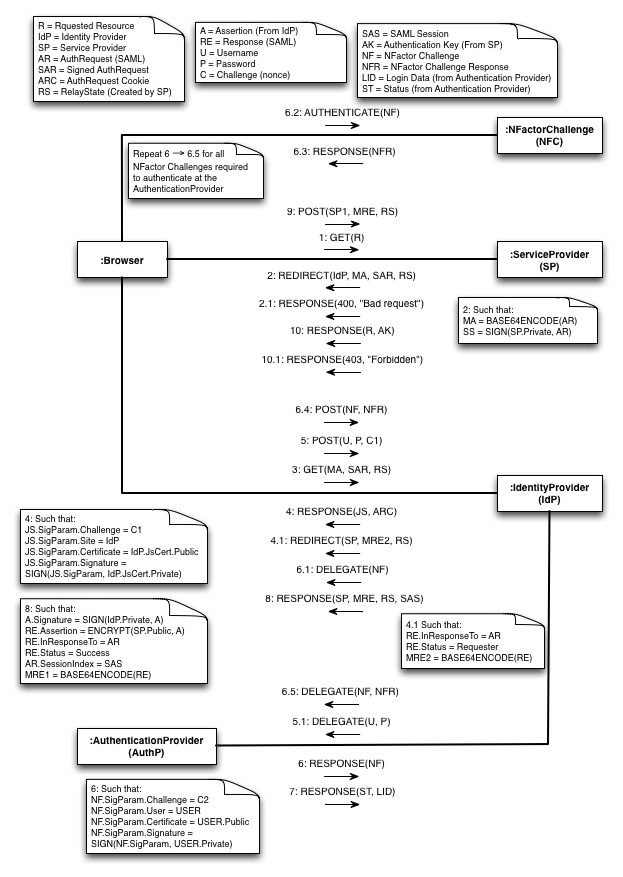
\includegraphics[scale=0.6]{images/Communication.png}

TEXT DESCRIBING ALGORITHM 1
\begin{algorithm}[H]
	\caption{Process 1}
	\begin{algorithmic}
	\REQUIRE{GET is well-formed \AND IdP.Public \AND SP.Private}
	\IF{R exists}
		\STATE AR $\leftarrow$ CreateAuthnRequest()
		\STATE SAR $\leftarrow$ SIGN(AR, SP.Private)
		\STATE MA $\leftarrow$ UrlEnc(Base64Enc(DeflateCompress(AR)))
		\STATE RS $\leftarrow$ UrlEnc(Base64Enc(R))
		\RETURN REDIRECT(IdP, MA, SAR, RS)
	\ELSE
		\RETURN RESPONSE(400, Bad−Request)
	\ENDIF
	\end{algorithmic}
\end{algorithm}

TEXT DESCRIBING ALGORITHM 2
\begin{algorithm}[H]
	\caption{Process 3}
	\begin{algorithmic}
		\REQUIRE{GET is well-formed \AND IdP.Private \AND SP.Public \AND IdPJsCert.Public \AND IdP has JavaScript from AuthP}
		\STATE AR $\leftarrow$ DeflateDecompress(Base64Dec(UrlDec(MA)))
		\IF{VERIFY(AR, SAR, SP.Public)}
			\STATE C1 $\leftarrow$ GenChallenge()
			\STATE JS $\leftarrow$ StoredJavaScript()
			\STATE JS.SigParams.Challenge $\leftarrow$ C1
			\STATE JS.SigParams.Certificate $\leftarrow$ IdPJsCert.Public
			\STATE JS.SigParams.Signature $\leftarrow$ SIGN(JS.SigParams, IdPJsCert.Private)
			\RETURN RESPONSE(JS)
		\ELSE
			\STATE RE $\leftarrow$ CreateResponse()
			\STATE RE.InResponseTo $\leftarrow$ AR
			\STATE RE.Status $\leftarrow$ ”Requester”
			\STATE MRE $\leftarrow$ Base64Enc(RE)
			\RETURN REDIRECT(SP, MRE, RS)
		\ENDIF
	\end{algorithmic}
\end{algorithm}

TEXT DESCRIBING ALGORITHM 3
\begin{algorithm}[H]
	\caption{Process 4}
	\begin{algorithmic}
		\REQUIRE{U \AND P \AND Browser allows JavaScript}
		\STATE SigParams $\leftarrow$ Js.SigParams
		\IF{VERIFY(SigParams, SigParams.Signature, SigParams.Certificate)}
			\STATE C1 $\leftarrow$ SigParams.Challenge
			\RETURN POST(U, P, C1)
		\ELSE
			\PRINT ERROR
		\ENDIF
	\end{algorithmic}
\end{algorithm}

TEXT DESCRIBING ALGORITHM 4
\begin{algorithm}[H]
	\caption{Process 5}
	\begin{algorithmic}
		\REQUIRE{POST is well formed}
		\IF{C1 matches challenge issued by IdP}
			\STATE \textbf{Delegate} U \AND P \TO AuthP
		\ELSE
			\RETURN RESPONSE(ERROR)
		\ENDIF
		\REQUIRE{C1 matches challenge issued by IdP}
	\end{algorithmic}
\end{algorithm}

TEXT DESCRIBING ALGORITHM 5
\begin{algorithm}[H]
	\caption{Process 5.1}
	\begin{algorithmic}
		\STATE USER $\leftarrow$ GetUser(U, P)
		\IF{USER is valid}
			\STATE C2 $\leftarrow$ GenChallenge()
			\STATE NF $\leftarrow$ GetNextNFactorChallenge(USER)
			\STATE NF.SigParam.User $\leftarrow$ USER
			\STATE NF.SigParam.Challenge $\leftarrow$ C2
			\STATE NF.SigParam.Certificate $\leftarrow$ USER.Public
			\STATE NF.SigParam.Signature $\leftarrow$ SIGN(NF.SigParam, USER.Private)
			\RETURN RESPONSE(NF)
		\ELSE
			\RETURN RESPONSE(ERROR)
		\ENDIF
	\end{algorithmic}
\end{algorithm}

TEXT DESCRIBING ALGORITHM 6
\begin{algorithm}[H]
	\caption{Process 6}
	\begin{algorithmic}
		\STATE SigParams $\leftarrow$ NF.SigParams
		\IF{VERIFY(SigParams, SigParams.Signature, SigParams.Certificate)}
			\STATE RELATE(SigParams.User, SigParams.Challenge)
			\STATE \textbf{Delegate} NF \TO Browser
		\ELSE
			\STATE \textbf{Delegate} ERROR \TO Browser
		\ENDIF
	\end{algorithmic}
\end{algorithm}

TEXT DESCRIBING ALGORITHM 7
\begin{algorithm}[H]
	\caption{Process 6.1}
	\begin{algorithmic}
		\STATE SigParams $\leftarrow$ NF.SigParams
		\IF{VERIFY(SigParams, SigParams.Signature, SigParams.Certificate)}
			\STATE AUTHENTICATE(NF)
		\ELSE
			\PRINT ERROR
		\ENDIF
	\end{algorithmic}
\end{algorithm}

TEXT DESCRIBING ALGORITHM 8
\begin{algorithm}[H]
	\caption{Process 6.2}
	\begin{algorithmic}
		\STATE NFR $\leftarrow$ NFactorResult(NF)
		\RETURN RESPONSE(NFR)
	\end{algorithmic}
\end{algorithm}

TEXT DESCRIBING ALGORITHM 9
\begin{algorithm}[H]
	\caption{Process 6.5}
	\begin{algorithmic}
		\REQUIRE{Stored relation for (NF.SigParams.USER, NF.SigParams.Certificate)}
		\STATE SigParams $\leftarrow$ NF.SigParams
		\IF{VERIFY(SigParams, SigParams.Signature, SigParams.Certificate)}
			\IF{NFR is acceptable result of NF}
				\STATE USER $\leftarrow$ GetUser(SigParams.USER, SigParams.Certificate)
				\STATE C2 $\leftarrow$ GenChallenge()
				\IF{USER.HasNextChallenge}
					\STATE NF $\leftarrow$ GetNextNFactorChallenge(USER)
					\STATE NF.SigParams.User $\leftarrow$ USER
					\STATE NF.SigParams.Challenge $\leftarrow$ C2
					\STATE NF.SigParams.Certificate $\leftarrow$ USER.Public
					\STATE NF.SigParams.Signature $\leftarrow$ SIGN(NF.SigParams, USER.Private)
					\RETURN RESPONSE(NF)
				\ELSE
					\STATE LID $\leftarrow$ CreateLogInData()
					\STATE ST $\leftarrow$ ”OK”
					\RETURN RESPONSE(ST, LID)
				\ENDIF
			\ELSE
				\RETURN RESPONSE(ERROR)
			\ENDIF
		\ELSE
			\RETURN RESPONSE(ERROR)
		\ENDIF	
	\end{algorithmic}
\end{algorithm}

TEXT DESCRIBING ALGORITHM 10
\begin{algorithm}[H]
	\caption{Process 7}
	\begin{algorithmic}
		\REQUIRE{SP.Public \AND LID is well-formed \AND stored AuthRequest for (LID.User, LID.Challenge)}
		\IF{ST = "OK"}
			\STATE ARC $\leftarrow$ GetAuthRequest(LID.User, LID.Challenge)
			\STATE MA $\leftarrow$ ARC.AR
			\STATE SAR $\leftarrow$ ARC.SAR
			\STATE RS $\leftarrow$ ARC.RS
			\STATE AR $\leftarrow$ DeflateDecompress(Base64Dec(UrlDec(MA)))
			\IF{VERIFY(AR, SAR, SP.Public)}
				\STATE A $\leftarrow$ BuildAssertion(LID.Certificate)
				\STATE SI $\leftarrow$ GenerateSessionIndex()
				\STATE A.InResponseTo $\leftarrow$ AR
				\STATE A.Issuer $\leftarrow$ IdP
				\STATE A.Audience $\leftarrow$ SP
				\STATE A.SessionIndex $\leftarrow$ SI
				\STATE A.Signature $\leftarrow$ SIGN(A, IdP.Private)
				\STATE EA $\leftarrow$ ENCRYPT(A, SP.Public)
				\STATE RE $\leftarrow$ CreateResponse()
				\STATE RE.Assertion $\leftarrow$ EA
				\STATE RE.InResponseTo $\leftarrow$ AR
				\STATE RE.Status $\leftarrow$ "Success"
				\STATE MRE $\leftarrow$ DeflateCompress(Base64Enc(UrlEnc(RE)))
				\STATE SAS $\leftarrow$ CreateSAMLSession(SI, SP, LID.CertificateSubject)
				\RETURN REDIRECT(SP, MRE, RS, SAS)
			\ELSE
				\STATE RE $\leftarrow$ CreateResponse()
				\STATE RE.InResponseTo $\leftarrow$ AR
				\STATE RE.Status $\leftarrow$ "Requester"
				\STATE MRE $\leftarrow$ DeflateCompress(Base64Enc(UrlEnc(RE)))
				\RETURN REDIRECT(SP, MRE, RS)
			\ENDIF	
		\ELSE
			\RETURN RESPONSE(ST)
		\ENDIF
	\end{algorithmic}
\end{algorithm}

TEXT DESCRIBING ALGORITHM 11
\begin{algorithm}[H]
	\caption{Process 9}
	\begin{algorithmic}
		\REQUIRE{POST is well.formed \AND SP.Private \AND IdP.Public}
		\STATE RE $\leftarrow$ UrlDec(Base64Dec(DeflateDecompress(MRE)))
		\STATE A $\leftarrow$ DECRYPT(RE.Assertion, SP.Private)
		\IF{VERIFY(A, A.Signature, IdP.Public)}
			\STATE AK $\leftarrow$ GenAuthKey()
			\STATE R $\leftarrow$ Base64Dec(UrlDec(RS))
			\STATE RES $\leftarrow$ GetResource(R)
			\RETURN RESPONSE(RES, AK)
		\ELSE
			\RETURN RESPONSE(403, Forbidden)
		\ENDIF
	\end{algorithmic}
\end{algorithm}

\chapter{F*}

This is F* code, doesn't it look pretty?
\newpage
%\begin{shaded}
\begin{lstlisting}[style=fstar, caption={ServiceProvider Module}]
	module Serviceprovider
	
	open SamlProtocol
	open Crypto
	
	val serviceprovider:  me:prin -> client:prin -> idp:prin -> unit
	
	let rec serviceprovider me client idp = 
	 let req = ReceiveSaml client in
	 match req with
	  | SPLogin (url) ->
	    let authnReq = CreateAuthnRequestMessage me idp in
	    assume(Log me authnReq);
	    let myprivk = CertStore.GetPrivateKey me in
	    let sigSP = Sign me myprivk authnReq in
	    let resp = AuthnRequestMessage me idp authnReq sigSP in 
	    SendSaml client resp;
	    serviceprovider me client idp
		(* This is awesome comment *)
	  | AuthResponseMessage (issuer, destination, encassertion) -> 
	    let myprivk = CertStore.GetPrivateKey me in
	    let assertion = DecryptAssertion me myprivk encassertion in
	    match assertion with
	    | SignedAssertion (token,sigIDP) ->
	      let pubkissuer = CertStore.GetPublicKey idp in
	      if VerifySignature idp pubkissuer token sigIDP
	      then
	        (assert(Log idp token);
	        let resp = LoginResponse "You are now logged in" in
	        SendSaml client resp)
	      else SendSaml client (DisplayError 403);
	      serviceprovider me client idp
	  
	  | _ -> SendSaml client (DisplayError 400);
	        serviceprovider me client idp
\end{lstlisting}
%\end{shaded}

\end{document}